%!TEX encoding = UTF-8 Unicode
\documentclass[a4paper]{article}

\usepackage{color}
\usepackage{url}
\usepackage[T2A]{fontenc} % enable Cyrillic fonts
\usepackage[utf8]{inputenc} % make weird characters work
\usepackage{graphicx}

\usepackage[english,serbian]{babel}
%\usepackage[english,serbianc]{babel} %ukljuciti babel sa ovim opcijama, umesto gornjim, ukoliko se koristi cirilica

\usepackage[unicode]{hyperref}
\hypersetup{colorlinks,citecolor=green,filecolor=green,linkcolor=blue,urlcolor=blue}

\usepackage{listings}
\usepackage{booktabs}

%\newtheorem{primer}{Пример}[section] %ćirilični primer
\newtheorem{primer}{Primer}[section]

\definecolor{mygreen}{rgb}{0,0.6,0}
\definecolor{mygray}{rgb}{0.5,0.5,0.5}
\definecolor{mymauve}{rgb}{0.58,0,0.82}

\lstset{ 
  backgroundcolor=\color{white},   % choose the background color; you must add \usepackage{color} or \usepackage{xcolor}; should come as last argument
  basicstyle=\scriptsize\ttfamily,        % the size of the fonts that are used for the code
  breakatwhitespace=false,         % sets if automatic breaks should only happen at whitespace
  breaklines=true,                 % sets automatic line breaking
  captionpos=b,                    % sets the caption-position to bottom
  commentstyle=\color{mygreen},    % comment style
  deletekeywords={...},            % if you want to delete keywords from the given language
  escapeinside={\%*}{*)},          % if you want to add LaTeX within your code
  extendedchars=true,              % lets you use non-ASCII characters; for 8-bits encodings only, does not work with UTF-8
  firstnumber=1000,                % start line enumeration with line 1000
  frame=single,	                   % adds a frame around the code
  keepspaces=true,                 % keeps spaces in text, useful for keeping indentation of code (possibly needs columns=flexible)
  keywordstyle=\color{blue},       % keyword style
  language=C,                      % the language of the code
  morekeywords={*,...},            % if you want to add more keywords to the set
  numbers=left,                    % where to put the line-numbers; possible values are (none, left, right)
  numbersep=5pt,                   % how far the line-numbers are from the code
  numberstyle=\tiny\color{mygray}, % the style that is used for the line-numbers
  rulecolor=\color{black},         % if not set, the frame-color may be changed on line-breaks within not-black text (e.g. comments (green here))
  showspaces=false,                % show spaces everywhere adding particular underscores; it overrides 'showstringspaces'
  showstringspaces=false,          % underline spaces within strings only
  showtabs=false,                  % show tabs within strings adding particular underscores
  stepnumber=2,                    % the step between two line-numbers. If it's 1, each line will be numbered
  stringstyle=\color{mymauve},     % string literal style
  tabsize=2,	                   % sets default tabsize to 2 spaces
  title=\lstname                   % show the filename of files included with \lstinputlisting; also try caption instead of title
}

\begin{document}

\title{Optimizacije - ključ dobrih performansi\\ \small{Seminarski rad u okviru kursa\\Metodologija stručnog i naučnog rada\\ Matematički fakultet}}

\author{Tamara Stojković, Emilija Stošić, Teodora Isailović \and tamara.stojkovic.1998@gmail.com, emilijazstosic@gmail.com, \and teodora.isailovic@gmail.com}
\date{12.~novembar 2022.}

\maketitle

\abstract{
Optimizacije su važan deo u procesu poboljšanja performansi programa. Kompajleri imaju različite nivoe optimizacije. Koji kompajleri i koji nivoi optimizacije će se koristiti zavisi od programa koji se kompajlira. Važno je razumeti sličnosti i razlike između optimizacija koje su dostupne u okviru savremenih kompajlera. U ovom radu ćemo predstaviti vrste optimizacija, sa akcentom na one koje su dostupne u okviru kompajlera GCC, LLVM i Native Image. }
\tableofcontents

\newpage

\section{Uvod}
\label{sec:uvod}
Optimizacija predstavlja tehniku transformacije dela programa,  tako da kod bude što je moguće efikasniji. 
Za cilj ima poboljšanje performansi koda, a ne savršen rezultat (uglavnom se ne može se reći da predstavlja pronalazak „optimalnog rešenja“ ). 
Optimizacija je oblast u kojoj se danas vrši većina istraživanja kompajlera. 
U okviru savremenih kompajlera dostupan je veliki broj optimizacija koje sve međusobno deluju na razne načine i imaju uticaj na kvalitet koda, veličinu koda, vreme kompilacije, potrošnju energije itd. 
Kompajleri obično obezbeđuju ograničen broj  standardnih optimizacionih nivoa, kao što su -O1, -O2,-O3 i -Os. Na ovim nivoima ostvaruju se kompromisi između  različitih mera kao što su kvalitet koda, veličina koda i vreme kompilacije. \cite{uvod}

\section{Osnovna podela optimizacija}
\label{sec:podela}
Postoje razne tehnike u primeni procesa optimizacije. Razlikujemo optimizacije koje se primenjuju na međukod,  kao deo generisanja ciljnog koda, ali i nakon generisanja ciljnog koda.
\textbf{Optimizacija međukoda} primenjuje se da se kod pojednostavi, preuredi ili sažme. Predstavlja optimizaciju koja ne uzima u obzir specifičnost ciljne arhitekture.
Neke od stavki koje \textbf{optimizacija kao deo generisanja ciljnog koda} omogućava su biranje instrukcija i određivanje načina alociranja objekata. Na kraju, može se izvršiti i \textbf{optimizacija ciljnog koda}, gde se pokušava prerada samog asemblerskog koda u nešto efikasnije. 
U ovom slučaju zahteva se deta\-ljno poznavanje ciljne arhitekture, kao i asemblerskog i mašinskog jezika ciljnog programa. \cite{osnovnaPodela}


\subsection{Optimizacije međukoda}
\label{subsec:optimizacija_međukod}
U okviru optimizacije međukoda razlikujemo: \textbf{lokalne}, \textbf{globalne} i \textbf{međuproceduralne optimizacije}.

\subsubsection{Lokalne optimizacije}
\label{subsubsec:lokalne}
Lokalne optimizacije služe za ubrzavanje malih delova neke funkcije i rade sa konketnim naredbama unutar osnovnog bloka (eng. ~{\em  Control - flow}).
One su obično najlakše za izvođenje jer nije neophodno raditi analizu kontrole toka (eng. ~{\em  Control - flow}).  
U nastavku navodimo neke od tehnika lokalne optimizacije koje se vrše nad međukodom. 

\begin{itemize}
  \item \textbf{Eliminacija čestih podizraza (eng. ~{\em Common subexpression elimination} )} \newline
  Podrazumeva izbegavanje izračunavanja čestog izraza više puta (ako se javlja više od jednom). 
  U slučaju da dve operacije daju isti rezu\-ltat, kažemo da su česte, pa je bolje izračunati izraz jednom i pozvati ga naredni put na mestu gde je neophodno.

  \item \textbf{Slaganje konstanti (eng. ~{\em Constant folding})} \newline
  Podrazumeva da se konstantni izrazi mogu evaluirati u vreme kompilacije. To uključuje utvrđivanje da svi operandi u izrazu imaju konstantnu vrednost, a zatim menjanje izraza njegovom vrednošću.
  Često je i lepše za pisanje i čitanje. 
  \item \textbf{Propagacija kopija (eng. ~{\em Copy propagation})} \newline
  Podrazumeva izbegavanje uvođenja promenljivih, koje samo čuvaju vrednosti nekih promenljivih koje već postoje.
  Posebno je značajna jer je u stanju da eliminiše veliki broj instrukcija, koje služe samo za kopiranje vrednosti iz jedne promenljive u drugu.
  \item \textbf{Smanjenje snage operatora (eng. ~{\em Operator strength reduction})} \newline
  Podrazumeva zamenu operatora „jeftinijim operatorom“. 
  Od same arhitekture zavisi koje operacije se smatraju najjeftinijim, a koje najskupljim, tako da je za dobru optimizaciju neophodno poznavati ciljnu mašinu.
  \item \textbf{Eliminacija mrtvog koda (eng. ~{\em Dead code elimination})} \newline
  Podrazumeva da ako se rezultat neke instrukcije nadalje ne koristi, instrukcija se smatra „mrtvom“ i može biti uklonjena. 
  Ovo omogućava uprošćavanje koda, izbacivanjem nepotrebnih izračunavanja.
  \item \textbf{Algebarsko pojednostavljenje i reasocijacija (eng. ~{\em Algebaric simplification and reassociation})} \newline
  Podrazumeva pojednostavljenje izraza korišćenjem algebarskih svojstava (zakona algebre). Reasocijacija podrazumeva korišćenje svojstava kao što su asocijativnost, komutativnost i distributivnost kako bi se nakon toga omogućila lakša primena drugih optimizacija.
  \item \textbf{Kompozicija lokalnih transformacija} \newline
  Različite optimizacije koje smo do sada videli, brinu o malom delu koda. 
  Za maksimalan efekat, možda će morati neke optimizacije da se primene više puta.  \cite{fogOptimizacije}

\end{itemize}



\subsubsection{Globalne optimizacije}
\label{subsubsec:globalne}
Predstavljaju optimizacije koje su slične lokalnim i koje možemo primeniti sa nekim dodatnim analizama.
„Globalno“ u ovom slučaju ne znači u celom programu, već se optimizacije primenjuju na jednu po jednu fu\-nkciju. 
Ova analiza je znatno moćnija od lokalne, ali dosta komplikovanija. 
Mnoge lokalne optimizacije mogu se primenjivati i globalno, dok postoje i one koje se mogu primeniti samo na globalnom nivou.
Neke globalne optimizacije date su u nastavku.

\begin{itemize}
  \item \textbf{Globalna eliminacija mrtvog koda} \newline
  U ovom slučaju jedina razlika je što se informacije o tome gde je neka promenljiva živa, moraju dobiti globalnom analizom, što je značajno komplikuje u odnosu na lokalnu eliminaciju mrtvog koda.
  \item \textbf{Globalno propagiranje konstante} \newline
  Ovo je optimizacija koja svaku promenljivu za koju se zna da je konstantna menja sa tom konstantom.
  Potrebno je pratiti vrednosti koje mogu biti dodeljene promenljivoj u svakoj tački programa. 
  \item \textbf{Globalna eliminacija čestih podizraza} \newline
  Česti podizrazi mogu se eliminisati  i na globalnom nivou, poznavanjem skupa dostupnih izraza.
  Izrazi su dostupni u jednom trenutku ako su živi pri ulasku u blok, što se utvrđuje ospežnom analizom.
  \item \textbf{Optimizacija kretanje koda (eng. ~{\em Code motion})} \\
  Postoje optimizacije koje se mogu primeniti samo globalno i jedna takva je ova i ona objedinjuje sekvence koda zajedničke za jedan ili više blokova. 
  Cilj je smanjiti veličinu koda i eliminisati eventualna skupa ponovna izračunavanja. 
  Dva oblika optimizacije izdizanjem koda koje ćemo izdvojiti su :
  \begin{itemize}
    \item \textbf{Pomeranje invarijantnog koda (eng. ~{\em loop-invariant})} \\
       Podrazumeva da se računanje vrednosti neke promenljive može izdvojiti izvan petlje, ako je nezavisno od brojača petlje.
    \item \textbf{Parcijalna eliminacija suvišnosti (eng. ~{\em Partial redundancy elimination})} \\
    Za neki račun u programu kaže se da je suvišan, ako računa već poznatu vrednost. 
    Parcijalno redundantno izračunavanje  je ono čija je vrednost poznata samo u nekim delovima. \cite{stanford}
    
  \end{itemize}
\end{itemize}


\subsubsection{Međuproceduralne optimizacije}
\label{subsubsec:međuproceduralne} 
U okviru ove optimizacije jedna od najznačajnijih tehnika je \textbf{uvlačenje definicija funkcija (eng. ~{\em Inlining})}. 
Uglavnom se jednostavnije funkcije uvlače, a složenije ne. 
Premalo uvlačenja dovodi do troškova vezanih za pozive funkcija, a previše uveća veličinu koda i dovodi do neefikasnosti, pa treba uspostaviti ravnotežu. \cite{kkFM}


\subsection{Optimizacije koda}
\label{subsec:optimizacija_kod}
Optimizovani međukod se u fazi generisanja koda prevodi u asemblerski tj. mašinski kod. 
U finalnom generisanju koda, bitno je donošenje pametnih odluka kako bi generisani ciljni kod bio što efikasniji. 
U ovom slučaju bitne su specifične karakteristike mašine za prozivodnju optimizovanog koda za tu konkretnu arhitekturu. 
Razlikujemo sledeće tehnike optimizacija koda :
\begin{itemize}
  \item \textbf{Optimizacija redosleda instrukcija} \\
  Razlikujemo fazu odabira instrukcija, fazu alokacije registara i fazu raspoređivanja instrukcija.
  \item \textbf{Optimizacija upotrebom keša} \\
  Upotreba keša se zasniva na prostornoj i vremenskoj lokalnosti, a cilj je da postane što bolja.
  Ako je nekoj memoriji skoro pristupano, vremenska podrazumeva da će biti uskoro opet, a prostorna da će i njeni susedni objekti biti uskoro korišćeni.
 
\end{itemize} 
Postoje razne optimizacije koje se mogu sprovesti i na nivou izgenerisanog ciljnog koda. \cite{kkMVJ}


\section{Napredne optimizacije u okviru kompajlera GCC/LLVM}
\label{sec:napredneOptimizacije}

\subsection{Optimizacije u okviru kompajlera GCC}
\label{subsec:optimizacijeGCC}

GCC je kompajler programskog jezika koji je razvio GNU, to je zvanični kompajler za GNU i Linux sisteme. Ričard Stolman (eng.~{\em Richard Stallman}) je 1984. godine pokrenuo GNU projekat čiji je cilj bio izgra\-dnja softverskog sistema otvorenog koda sličnog UNIKS-u. GNU operativni sistem se nije razvijao kako se očekivalo. Međutim, razvili su se mnogi odlični i korisni softverski alati otvorenog koda, kao što su Make, Emacs, GDB i GCC. \cite{gccVsClang}

GCC prevodi program, ukoliko nema sintaksnih grešaka, kreiraće se izvršni fajl, u suprotnom će prevodilac ispisati poruke o greškama i broj linija u kodu gde se te greške nalaze. Takođe, gcc ima veliki broj opcija kojima se mogu podesiti parametri prevođenja. Opcijom -o se zadaje ime izvršnog programa, opcije -Wall, -Wextra se koriste za generisanje poruka o upozorenjima, kada postoje konstrukcije koje su sintaksno ispravne, ali mogu da budu semantički neispravne. Opcije koje su vrlo značajne u procesu kompilacije, su opcije za optimizaciju. Kao i kod opcija za upozorenja i kod opcija za optimizaciju moguće je precizno definisati koje se sve optimizacije vrše ili se može zadati neka od grupnih opcija koje podržavaju veći broj optimizacija. Nivo optimizacije koju kompajler vrši se kontroliše opcijom -On, gde je n nivo zahtevane optimizacije. Promena ove vrednosti će zahtevati više vremena za kompilaciju koda i koristiće mnogo više memorije, posebno kako se povećava nivo optimizacije. \cite{gnuSamardzic} Neke optimizacije smanjuju veličinu rezultujućeg koda, dok druge pokušavaju da kreiraju brži kod, potencijalno povećavajući njegovu veličinu. Postoji osam -O podesavanja: \textbf{-O0, -O1, -O2, -O3, -Os, -Oz, -Og, -Ofast}.
\begin{itemize}
\item \textbf{O0 nivo optimizacije:} Na ovom nivou optimizacija je potpuno isključena. Ako se ne navede -O opcija, ovo je podrazumevani nivo optimizacije. Ovaj nivo značajno smanjuje vreme kompilacije i poboljšava informacije o otklanjanju grešaka. Neki programi ne rade ispravno bez nekog nivoa optimizacije, pa se ovaj nivo ne preporučuje.
\item \textbf{O1 nivo optimizacije:} Optimizacije koje se vrše na ovom nivou imaju dva cilja, koji nekad mogu da budu suprotstavljeni, smanjenje veličine koda koji se kompajlira, uz povećanje njegovih performansi. Optimizacije obično ne zahtevaju značajnu količinu vremena da bi se izvršile.
\item \textbf{O2 nivo optimizacije:} Preporučeni nivo optimizacije. Kompajler pokušava da poveća performanse koda bez ugrožavanja veličine samog koda i bez uzimanja previše vremena za kompilaciju.
\item \textbf{O3 nivo optimizacije:} Ovo je najviši nivo optimizacije. Na ovom nivou naglasak je na brzini kompajliranja, a ne na veličini generisanog koda. Ovde je omogućena i optimizacija inline-funkcija, što povećava performanse, ali može da poveća veličinu samog koda, što zavisi od veličine funkcija koje su umetnute. Kompajliranje na ovom nivou ne garantuje povećanje performansi, zapravo, često sistem može da se uspori zbog većih binarnih datoteka i povećane upotrebe memorije. Ovaj nivo optimizacije se ne preporučuje.
\item \textbf{Os nivo optimizacije:} Na ovom nivou se vrše sve optimizacije kao i na nivou -O2, koje ne povećavaju veličinu koda, kao što su optimizacije poravnanja. Ovde je stavljen naglasak na veličinu, a ne na brzinu generisanog koda.
\item \textbf{Og nivo optimizacije:} Ovaj nivo optimizacije je uveden u 4.8 standardu. Na ovom nivou naglasak je na brzini kompajliranja i na otklanjanju grešaka, dok se istovremeno pruža određeni nivo performansi.
\item \textbf{Ofast nivo optimizacije:} Ovaj nivo je uveden u 4.7 standardu. Na ovom nivou se vrše sve optimizacije kao i na nivou -O3 plus \textbf{-ffast-math, -fno-protect-parens i -fstack-arrais}. \cite{gccOptions}
\end{itemize}

Naredni program se koristi za demonstraciju efekata različitih nivoa optimizacije :
\newpage
\begin{lstlisting}
#include <stdio.h>

double powern (double d, unsigned n)
{
  double x = 1.0;
  unsigned j;
  for (j = 1; j <= n; j++)
    x *= d;
  return x;
}

int main (void)
{
  double sum = 0.0;
  unsigned i;
  for (i = 1; i <= 100000000; i++) {
      sum += powern (i, i % 5);
  }
  printf ("sum = %g\n", sum);
  return 0;
}
\end{lstlisting}

Glavni program sadrži petlju koja poziva funkciju powern, koja računa n-ti stepen broja. Vreme izvršavanja programa se može meriti naredbom time. Sa slike \ref{fig:Rezultati_optimizacije} se jasno vidi da se brzina izvršavanja programa povećava, kako se povećava nivo optimizacije.

\begin{figure}[h!]
    \begin{center}
        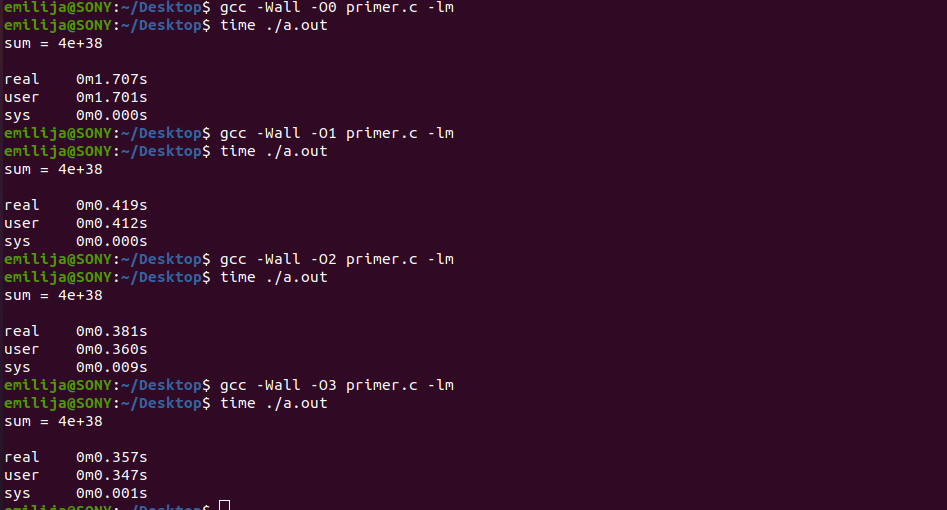
\includegraphics[width=105mm, height=30mm]{pics/test.png}
    \end{center}
    \caption {Rezultati optimizacije}
    \label{fig:Rezultati_optimizacije}

\end{figure}


\subsection{Optimizacije u okviru kompajlera LLVM}
\label{subsec:optimizacijeLLVM}

LLVM je projakat otvorenog koda koji je razvio Kris Latner (eng.~{\em Chris Lattner}), kao istraživački projekat na Univerzitetu Ilinois. LLVM je zvanični naziv koji je primenljiv na sve projekte pod LLVM, koji zajedno čine potpun kompajler : prednji, srednji i zadnji deo, optimizatore, asemblere, linkere, libc++ i druge komponente. Pomaže u izgradnji novih računarskih jezika i poboljšanju postojećih. Automatizuje teške i neprijatne zadatke koji su uključeni u kreiranje jezika, kao što je prenos izlaznog koda na više platformi i arhitektura, LLVM je zapravo okvir za generisanje objektnog koda iz bilo koje vrste izvornog koda. LLVM ne vrši samo kompajliranje IR u izvorni mašinski kod, takođe može da vrši optimizaciju koda. Optimizacije mogu biti prilično agresivne, uključujuci stvari kao što su umetanje funkcija, eliminisanje mrtvog koda i odmotavanje petlji. \cite{llvm1} \cite{gccVsClang}

Alat opt vrši analizu i optimizaciju koda. Uzima ulazne llvm datoteke kao ulaz, pokreće optimizacije ili analize i na kraju vraća optimizovanu datoteku ili rezultate analize. Ukoliko je zadata opcija -analyze, opt pokreće različite analize nad ulazom. Ukoliko opcija  -analize nije data, opt vrši optimizacije i pokušava da proizvede optimizovanu izlaznu datoteku. Optimizacije su zadate u vidu prolaza, koji prelaze neki deo programa da bi prikupili informacije ili transformisali program. Alat opt može da pokrene samo odabrane optimizacije, u određenom redosledu, tako što se pri pokretanju alata zadaju imena tih prolaza u željenom redosledu. Svi LLVM prolazi su podklase klase Pass, funkcionalnosti prolaza su implementirane tako što prevazilaze virtuelne metode nasleđene od klase Pass. Analysis Passes se koriste za prikupljanje informacija koje mogu da služe za otklanjanje grešaka ili vizuelizaciju programa. Transform Passes se koriste za optimizaciju koda. Utility Passes služe za dobijanje raznih informacija, koje su bitne za razvoj drugih prolaza. Nakon svakog prolaza IR mora da bude u validnom stanju.

Postoji sedam -O nivoa optimizacije : 
\begin{itemize}
\item \textbf{O0 nivo optimizacije :} Na ovom nivou, optimizacija je potpuno isključena. Ovo je podrazumevani nivo optimizacije i na ovom nivou kod se najbrže kompajlira.
\item \textbf{O1 nivo optimizacije :} Najosnovniji nivo optimizacije.
\item \textbf{O2 nivo optimizacije :} Na ovom nivou je omogućena većina optimizacija, ovo je preporučeni nivo optimizacije.
\item \textbf{O3 nivo optimizacije :} Na ovom nivou su dozvoljene sve optimizacije kao i na nivou -O2, sa dodatnim optimizacijama koje mogu generisati veći kod u cilju da se program brže pokrene.
\item \textbf{O4 nivo optimizacije :} Ovo je najviši nivo optimizacije. Optimizacija celog programa se vrši u vreme povezivanja. 
\item \textbf{Os nivo optimizacije :} Ovaj nivo optimizacije podržava sve optimizacije kao i nivo -O2, sa dodatnim optimizacijama za smanjenje veličine koda.
\item \textbf{Oz nivo optimizacije :} Na ovom nivou su dozvoljene sve optimizacije kao i na nivou -Os, a samim tim i -O2,  sa dodatnim smanjenjem veličine koda. \cite{opt} \cite{pass} \cite{pass2}
\end{itemize}


\section{Različite optimizacije u okviru kompajlera GCC/LLVM}
\label{subsec:razlike}

U odnosu na namenu svakog od ovih kompajlera  i opseg programa za koje su specifikovani, određuje se i koji je bolji za optimizaciju u nekim konkretnim slučajevima.
Karakteristike kompajlera koje određuju njihovu oblast upotrebe pa samim tim i optimizacije su : 
\begin{itemize}
  \item \textbf{GCC} podržava tradicionalne jezike kao što su Ada, Fortran i GO.
         GCC podržava manje popularne arhitekture, kao i RISC-V ranije u odnosu na LLVM.
         Trenutno je brži od LLVM-a u  kompajliranju LINUX kernela. 
         U slučaju korišćenja LLVM-a, kernel se ne može kompajlirati bez modifikacije izvornog koda i parametara kompilacije.
  \item  Novi jezici  kao što su Swift, Rust, Julia i Ruby, koriste \textbf{LLVM}.
          LLVM je usklađen strožije sa standardima C-a i C++-a nego GCC, pa se problemi manje javljaju.
          On takođe podržava neke ekstenzije, kao što su atributi za proveru bezbednosti niti.
          Ovaj kompilator omogućava tačnije i preciznije dijagnostičke informacije i poruke o greškama. U GCC-u su počele da se poboljšavaju od GCC-a 8.
          Clang obezbeđuje dodatne korisne alate za statičku analizu i skeniranje koda (scan-build, clang static analyzer, clang-format, clang-tidy).
          Clang je kompajler  za C, C++, Objective-C, ili Objective-C++.
\end{itemize}
GCC se smatrao superiornijim, ali LLVM napreduje. Sada neki smatraju da se LLVM uglavnom koristi da obezbedi performanse superiornije od GCC-a.
\\ Optimizacije su do sada postale jedna od osnovnih komponenti kompa\-jlera. 
U kompajlerima je implementirano stotine optimizacija. 
Na primer, postoji više od 200 optimizacija za GCC i više od 100 za LLVM.  
Rezultati optimizacije u okviru ovih kompajlera najčešće se moraju posmatrati na konkretnim slučajevima, pa  su neki primeri dati u nastavku.

\subsection{Prvi primer testiranja razlika}
\label{subsec:primer1}
Većina radnih opterećenja u oblaku (eng. ~{\em cloud workloads}) mogu da rade u različitim klasterima i nije potrebno navoditi parametre koji se odnose na mašinu. 
Samo radno opterećenje ima nizak nivo kompilacije i optimizacije (-O2 ili ispod).
Posmatranjem razlika za GCC i LLVM na nivoima -O2 i -O3 za INT Speed programe (za testiranje brzine) utvrđeno je da 
GCC ima prednost od 1\% do 4\% u odnosu na LLVM u slučaju većine programa na nivoima -O2 i -O3. 
Stavke koje su uzete za test nemaju specifične žarišne tačke, pa se mogu smatrati sveobuhvatnim.

Iz ovog testiranja se mogu izvesti sledeća zapažanja : 

\begin{itemize} 
\item Rezultati testiranja pokazuju da je GCC uvek povoljan u pogledu optimizacije performansi. 
Međutim u 2 specifična programa u vezi sa veštačkom inteligencijom LLVM poboljšava performanse za više od 3\% u odnosu na GCC. 
\item LLVM optimizuje vektore na nivou -O2,  a GCC na -O3 nivou. 
\item Osim vektorizovanih programa, GCC ne poboljšava performanse na nivou -O3, u poređenju sa onim na -O2, dok LLVM značajno poboljšava performanse nekih programa na nivou -O3. 
\item U nekim slučajevima (na nivoima -O3 i više) GCC može poboljšati performanse, dok Clang ima tendenciju da previše odmotava petlje, što može dovesti do problema (ovde je rešenje koristiti optimizovanje za veličinu (-Os) da biste ograničili odmotavanje petlji).
\end{itemize}

LLVM međukod je koncizniji i zauzima manje memorije tokom kompilacije od GCC međukoda.
Na osnovu urađenih testova, zaključeno je da Clang nudi više prednosti u procesu izgradnje velikih projekata nego GCC. 
GCC je skoro uvek povoljan u pogledu performansi, ali izbor ipak zavisi od specifične aplikacije. \cite{gccVsClang} 

\subsection{Drugi primer testiranja razlika}
\label{subsec:primer1}

U većini nabrojanih  vrsta optimizacija u sekciji \ref{sec:podela} kao što su uvlačenje definicija funkcija, slaganje konstanti, propagacija konstanti, na testiranom konkretnom primeru oba kompajlera pokazala su se dobro.

Neke razlike koje su primećene su : 
\begin{itemize}
\item Kod odmotavanja petlji niza (eng. ~{\em loop unroling, array loops}) LLVM ne funkcioniše ispravno i komplikuje, dok GCC dobro radi. 
\item U slučaju indukcionih promenljivih sa float izrazima  ili sa integer izrazima (koji nisu nizovi elemenata) GCC ne može da radi, a LLVM radi. Takođe važi i u slučaju više akumulatora (integer ili float).
\item U ovom slučaju GCC nije radio ni za algebarsku redukciju primenom asocijativnosti, dok LLVM jeste. \cite{fogOptimizacije}
\end{itemize}

\subsection{Razlike u nivoima optimizacije}
\label{subsec:nivoiRazlika}
Kompajleri GCC i LLVM imaju po sedam nivoa optimizacije, sa manjim ili većim razlikama. 
Optimizacije koje se vrše na nivoima -O0 i -O1 su identične. Kod gcc kompajlera nivo -O2 je preporučeni nivo optimizacije, dok je kod llvm kompajlera ovo umereni nivo optimizacije. -Os nivo optimizacije kod gcc kompajlera aktivira sve -O2 optimizacije koje ne povećavaju veličinu generisanog koda, dok kod llvm kompajlera ovaj nivo aktivira sve -O2 optimizacije koje smanjuju veličinu koda. -Oz i -O4 nivoi optimizacije postoje samo kod llvm kompajlera. -O4 nivo je najviši nivo optimizacije kod llvm kompajlera, dok je kod gcc kompajlera to -O3 nivo. Ovo nisu preporučeni nivoi optimizacije. Nivoi -Og i -Ofast se javljaju samo kod gcc kompajlera.
\\

\vspace{2em}
\hspace{-5em}
\begin{tabular}{|c|c|c|}
  \toprule
   & \textbf{GCC} & \textbf{LLVM} \\
  \midrule
  \textbf{Modularnost koda} & Monolitičan & Modularan \\
  \midrule
  \textbf{Generisani} & Efikasan, & Efikasan, zbog korišćenja \\
  \textbf{kod} & veliki broj opcija &  SSA forme na LLVM backend-u \\
  \midrule
  {} & Sporiji zbog oslanjanja  & Brži zbog integrisanja  \\  
  \textbf{Brzina} & na nezavisne kompajlere.  & sopstvenih kompajlera. \\  
  \textbf{kompilacije} & Nakon IR, asemblerski kod, & Objektni fajl direktno iz IR \\  
  {} & pa iz njega objektni fajl & objektni fajl direktno iz IR \\  
  \midrule
  \textbf{Brzina izvršavanja} &   \multicolumn{2}{|c|}{GCC u proseku brži 1-4\%  za većinu} \\
  \textbf{dobijenog koda}     &   \multicolumn{2}{|c|}{programa na 02 i 03 nivou}  \\  
  \bottomrule
  \end{tabular}

  \vspace{2em}
  

% Koje su razlike između optimizacija GCC/LLVM i kompajlera Native Image
\section{Native-Image kompajler}
\label{sec:natImg}

Neke od glavnih prednosti softvera pisanog u jezicima koji se prevode specifično platformi je
brzina pokretanja i manja količina neophodnih resursa. Takav softver se izvršava direktno na
procesoru, a ne na virtualnoj mašini (apstrakciji procesora).

Native-Image kompajleri predstavljaju tehniku ahead-of-time kompilacije od izvornog koda preko
bytecode-a do izvršivog koda određene platforme i arhitekture, koji se 
naziva \textbf{native image}. \cite{natImgGraal01}
Najpoznatiji primeri su \textit{Native Image} iz GraalVM za jezike na JVM i
\textit{Ngen} za .NET Framework, odnosno \textit{CrossGen} za .NET Core.
U nastavku opisan je alat iz GraalVM.

Proizvod je statički povezan kod koji se ne izvršava na VM, ali u sebi sadrži njene neophodne 
komponente poput garbage collector-a. Takođe, sadrži i klase i pakete,
runtime klase biblioteka i statički povezan mašinski kod. \cite{natImgGraal02}

Originalni, čisti izvorni kod se prevodi do bytecode-a na poznat način.
Image builder je zadužen za određivanje zavisnosti. Vrši se statička
analizira dosežnosti klasa i metoda. Sav dosežan kod se zatim 
kompajlira ahead-of-time za ciljani operativni sistem i arhitekturu.

\begin{figure}[h!]
  \begin{center}
      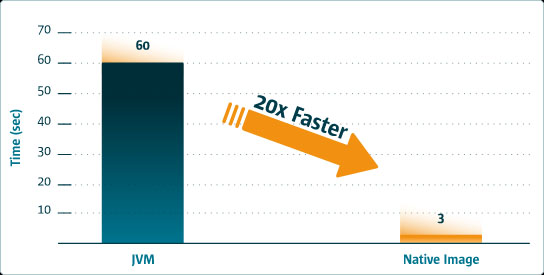
\includegraphics[width=70mm]{./pics/alibaba_pic.jpg}
  \end{center}
  \caption {GraalVM}
  \label{fig:natImg-alibaba}
\end{figure}

\subsection{Problemi i optimizacije}
\label{sec:natImg-proboptim}

Problem na koji se nailazi u nekim prilikama je nemogućnost 
primene ahead-of-time kompajliranja. U tom slučaju se pokreće 
agresivnije analiziranje korišćenjem pretpostavki (eng.~{\em closed-world optimization}). 
Na taj način sav dostižan kod biće poznat tokom prevođenja.
Ukoliko se kod ne može optimizovati, generiše se fallback slika
koja se pokreće na Java HotSpot VM. Da bi se izbegle ovakve situacije,
moguće je napraviti konfiguracioni fajl sa razrešenjem.

\subsubsection{Dinamičko učitavanje i refleksija}
\label{sec:natImg-dynRefl}
Svaka klasa kojoj se pristupa preko imena u runtime-u mora 
biti označena u build time-u.
Da bi se razrešili svi elementi kojima se pristupa reflektivno,
Native Image pokušava statičkom analizom da detektuje pozive 
iz Reflection API.

Dynamic Proxy su podržani ahead-of-time. Statička analiza 
jednostavno presreće pozive metoda newProxyInstance i 
getProxyClass i pokušava da automatski odredi listu interfejsa.

\subsubsection{Java Native Interface}
\label{sec:natImg-jni}
JNI omogućava native kodu da pristupa Java objektima, klasama,
metodama i poljima preko imena. Gledajući da je princip sličan
kao i korišćenje reflection API-a u Javi, neophodno je specificirati
generisanje slike u konfiguracionom fajlu.
Native image nudi svoj interfejs kao dopunu JNI.
On omogućava jeftiniju i jednostavniju alternativu JNI. Takođe
omogućava pozive između Java i C koda, kao i pristup C strukturama
podataka iz koda pisanog u Javi.



\section{Zaključak}
\label{sec:zakljucak}

Mnogi optimizacioni problemi su NP-kompletni (Np-teški ili neodlučivi), pa se samim tim većina algoritama za optimizaciju oslanja na aproksimaciju i heuristiku.  
I pored toga, algoritmi rade uglavnom prilično dobro. 
Programer ima jako veliku ulogu u dobijanju efikasnog koda, ali ako je algoritam koji se koristi loš, optimizacija ga ne može učiniti bržim. 
Bitno je napomenuti i da optimizacija ne bi trebalo da menja ispravnost koda. 
Očekuje se da program koji je optimizovan, daje iste izlaze, za iste ulaze, kao i početni neoptimizovani program.
Optimizacije u navedenim kompajlerima su ključna stvar za dostizanje dobrih performansi koda. 
Jedni drugima su uglavnom konkurencija, pa će kao i dosadašnje napredne optimizacije u okviru njih, i dalja istraživanja u ovoj 
oblasti biti usmerena ka poboljšanjima, kako rešavanjem njihovih nedosatataka, tako i mana u poređenju sa konkurentima.


\addcontentsline{toc}{section}{Literatura}
\appendix
\bibliography{seminarski} 
\bibliographystyle{plain}



\end{document}
